\documentclass[tikz,border=10pt]{standalone}
\usetikzlibrary{arrows.meta,positioning,calc,matrix}
\begin{document}
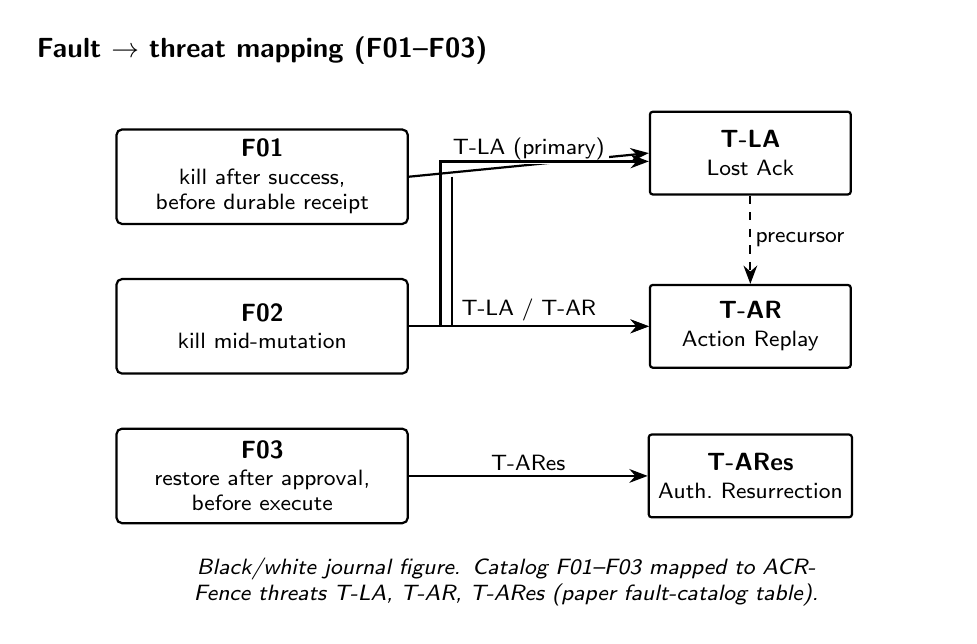
\begin{tikzpicture}[
  font=\sffamily\small,
  >=Stealth,
  fault/.style={draw, thick, rounded corners=2pt, align=center,
    minimum width=3.7cm, minimum height=1.2cm, fill=white},
  threat/.style={draw, thick, rounded corners=1pt, align=center,
    minimum width=2.55cm, minimum height=1.05cm, fill=white},
  el/.style={font=\sffamily\footnotesize, fill=white, inner sep=1.5pt}
]
  \node[font=\sffamily\bfseries] (title) at (0,4.2) {Fault $\to$ threat mapping (F01--F03)};

  % Left: faults
  \node[fault] (f01) at (0,2.6)
    {\textbf{F01}\\[-1pt]{\footnotesize kill after success,}\\[-2pt]{\footnotesize before durable receipt}};
  \node[fault] (f02) at (0,0.7)
    {\textbf{F02}\\[-1pt]{\footnotesize kill mid-mutation}};
  \node[fault] (f03) at (0,-1.2)
    {\textbf{F03}\\[-1pt]{\footnotesize restore after approval,}\\[-2pt]{\footnotesize before execute}};

  % Right: threats (spaced vertically)
  \node[threat] (tla) at (6.2,2.9)
    {\textbf{T-LA}\\[-1pt]{\footnotesize Lost Ack}};
  \node[threat] (tar) at (6.2,0.7)
    {\textbf{T-AR}\\[-1pt]{\footnotesize Action Replay}};
  \node[threat] (tares) at (6.2,-1.2)
    {\textbf{T-ARes}\\[-1pt]{\footnotesize Auth.\ Resurrection}};

  % F01 -> T-LA and T-AR (T-LA then AR)
  \draw[thick,->] (f01.east) -- node[el, above] {T-LA (primary)} (tla.west);
  \draw[thick,->] (f01.east) +(0.55,0) |- node[el, near end, above] {$\to$T-AR} (tar.west);

  % F02 -> T-LA and T-AR
  \draw[thick,->] (f02.east) -- node[el, above] {T-LA / T-AR} (tar.west);
  \draw[thick,->] (f02.east) +(0.4,0) |- ([yshift=-3pt]tla.west);

  % F03 -> T-ARes
  \draw[thick,->] (f03.east) -- node[el, above] {T-ARes} (tares.west);

  % T-LA precursor annotation
  \draw[thick,->,dashed] (tla.south) -- node[el, right] {precursor} (tar.north);

  \node[font=\sffamily\footnotesize\itshape, align=center, text width=11cm]
    at (3.1,-2.55)
    {Black/white journal figure. Catalog F01--F03 mapped to ACRFence threats
     T-LA, T-AR, T-ARes (paper fault-catalog table).};
\end{tikzpicture}
\end{document}
